\documentclass{standalone}
\usepackage{tikz}
\begin{document}

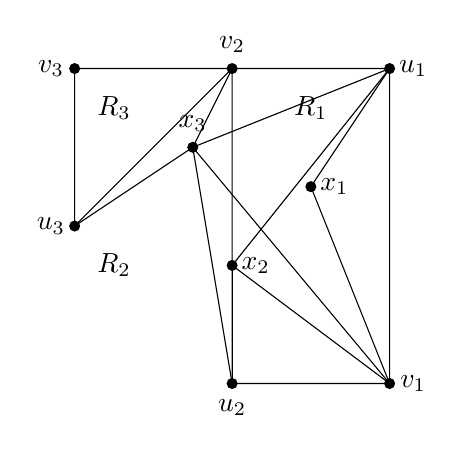
\begin{tikzpicture}

% Define coordinates
\coordinate (u1) at (2,2);
\coordinate (u2) at (0,-2);
\coordinate (u3) at (-2,0);
\coordinate (v1) at (2,-2);
\coordinate (v2) at (0,2);
\coordinate (v3) at (-2,2);
\coordinate (x1) at (1,0.5);
\coordinate (x2) at (0,-0.5);
\coordinate (x3) at (-0.5,1);

% Draw the hexagon
\draw (u1) -- (v1) -- (u2) -- (v2) -- (u3) -- (v3) -- cycle;

% Draw lines from x3
\draw (x3) -- (u1);
\draw (x3) -- (u2);
\draw (x3) -- (u3);
\draw (x3) -- (v1);
\draw (x3) -- (v2);

% Draw lines from x2
\draw (x2) -- (u1);
\draw (x2) -- (u2);
\draw (x2) -- (v1);

% Draw lines from x1
\draw (x1) -- (u1);
\draw (x1) -- (v1);

% Draw nodes
\foreach \point in {u1, u2, u3, v1, v2, v3, x1, x2, x3}
    \fill (\point) circle (2pt);

% Labels
\node at (2.3,2) {$u_1$};
\node at (0,-2.3) {$u_2$};
\node at (-2.3,0) {$u_3$};
\node at (2.3,-2) {$v_1$};
\node at (0,2.3) {$v_2$};
\node at (-2.3,2) {$v_3$};
\node at (1.3,0.5) {$x_1$};
\node at (0.3,-0.5) {$x_2$};
\node at (-0.5,1.3) {$x_3$};

% Region labels
\node at (1,1.5) {$R_1$};
\node at (-1.5,-0.5) {$R_2$};
\node at (-1.5,1.5) {$R_3$};

\end{tikzpicture}

\end{document}